% !TEX root = ../../teaching_online.tex
\newpage
\section{Blackboard}

% What is Blackboard
\subsection{What is Blackboard?}

Blackboard is an online website for instructors. It can be used for in-person or (synchronous or asynchronous) online teaching. Using Blackboard, you can send individual, group, or course emails, record grades, create or link to course content, administer quizzes and exams, and more. Note that all images in this section were taken from the Blackboard Instructor help pages.



% Blackboard Resources
\subsection{Essential Blackboard Resources}

        \begin{itemize}
        \item Blackboard Learn Help for Instructors: \url{https://help.blackboard.com/Learn/Instructor}
        
        \item Blackboard Learn---For Instructors YouTube Videos: \url{https://www.youtube.com/playlist?list=PLontYaReEU1tzu1T5gfiX-JQA5nBc3isN}
        
        \item Syracuse University IT Help: \url{https://its.syr.edu/get-help/}
        \end{itemize}


% Blackboard Quick Start
\subsection{Blackboard Quick Start}

The `Blackboard Learn---For Instructors YouTube Videos' link above is a great place to start learning how to do things in Blackboard. However, Blackboard has a `Quick Start' page for starting on Blackboard that is also worth examining. This page is found at \url{https://help.blackboard.com/Learn/Instructor/Quick_Start}.



% Logging In
\subsection{Logging into Blackboard}

You can login to Blackboard using \url{https://blackboard.syr.edu/}. You can also access Blackboard while logged into MySlice using the \its{Blackboard \@ SU} link under the \its{MySlice Applications} $\to$ \its{Academic Applications}. If you have trouble finding this, use the \its{Find} feature of your browser using Cntrl $+$ F (PC) or Cmmd $+$ F (Mac). 



% Making the Course Available
\subsection{Making the Course Available}

Making the course available to students is the last and most important step in setting up your Blackboard course. We present this first because it is easily missed or forgotten. 

\begin{enumerate}[1.]
\item \its{Control Panel} $\to$ \its{Customization} $\to$ \its{Properties} $\to$ \its{Set Availability}.
\item Set the \its{Make Course Available} under the \its{Set Availability} to \its{Yes}.
\item Click \its{Submit}.
\end{enumerate}

Note you can choose when the course becomes available/unavailable using the \its{Set Course Duration} options. You can always make a course unavailable and re-available. You can find more at \url{https://help.blackboard.com/Learn/Instructor/FAQ/Course_FAQs}.

	\begin{figure}[!ht]
	\centering
	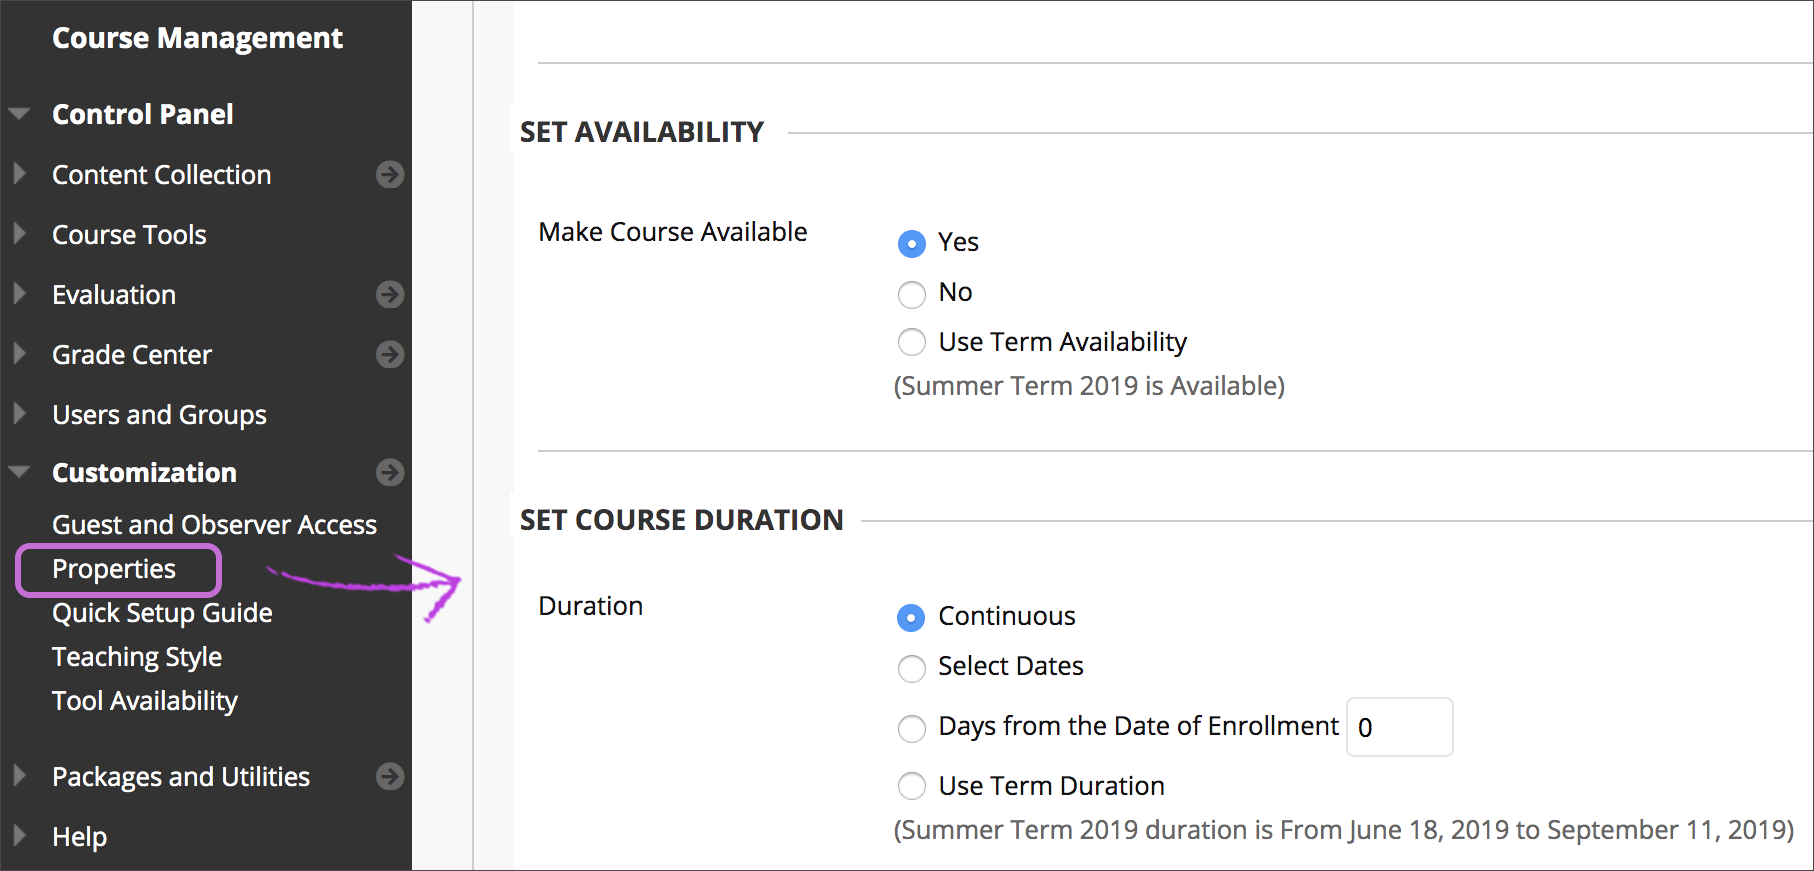
\includegraphics[width=1.1\textwidth]{sections/blackboard/images/original_course_availability.png}
	\caption{Making a Blackboard course available.}
	\end{figure}



% Taking Attendance
\subsection{Taking Attendance}

You can take attendance using Blackboard, and you can include it in your grade book. To access attendance:

	\begin{enumerate}[1.]
	\item \its{Control Panel} $\to$ \its{Course Tools} $\to$ \its{Attendance}.
	\item Select \its{Add Attendance}.
	\end{enumerate}

You mark attendance using Control Panel $\to$ Course Tools $\to$ Attendance. You can select the way that the attendance grade is displayed and what the point/percentage values are for \its{Present}, \its{Late}, and \its{Absent} are. Although, you may not be able to when you initially add taking attendance. But these settings can be changed in the \its{Settings} panel. Be sure to save your changes. 

	\begin{figure}[!ht]
	\centering
	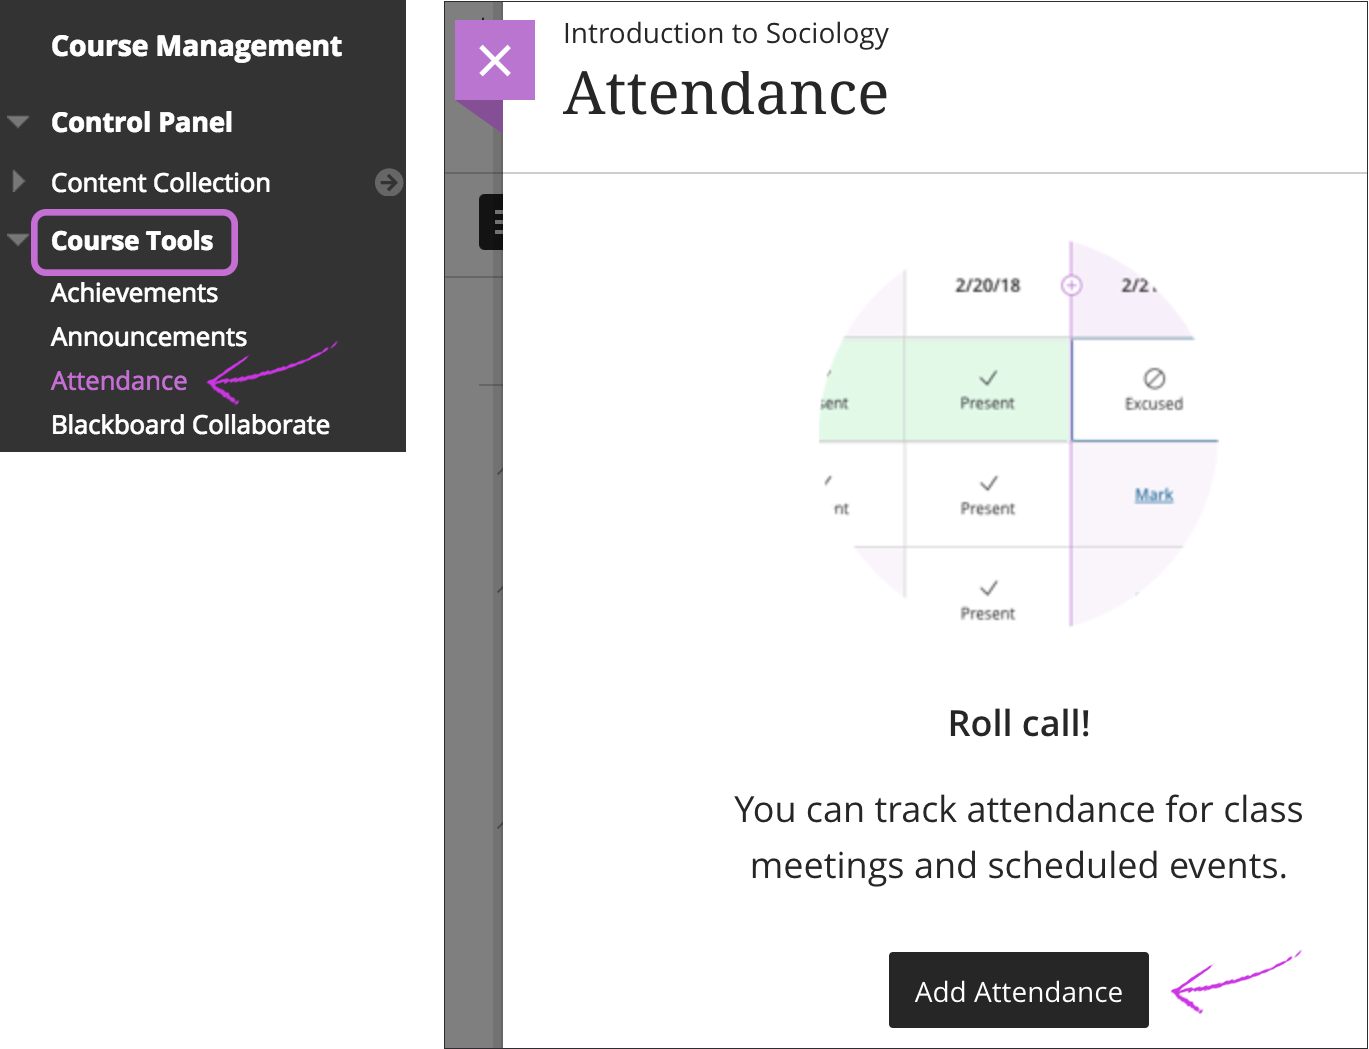
\includegraphics[width=0.7\textwidth]{sections/blackboard/images/learn_orig_instr_attendance_first_access_1_1.png}
	\caption{Adding attendance on Blackboard.}
	\end{figure}

You can also record students attendance for meetings as well as virtual classes via Blackboard Collaborate Ultra. In the \its{Overall} view, you can mark attendance, view your students attendance history and class statistics, and create meetings. Students can be exempted from classes or meetings. Note that if you alter an individual students attendance grade cell, the entered grade becomes the fixed percentage. It is better to alter individual class/meeting grade. Finally, you can export and import attendance records as well. More on all the attendance features as well as a brief overview for setting it up can be found below:

	\begin{itemize}
	\item Blackboard Attendance: \url{https://help.blackboard.com/Learn/Instructor/Grade/Attendance}
	\item Marking Attendance in Blackboard---YouTube: \url{https://www.youtube.com/watch?v=C9FCxq1hfUY}
	\end{itemize}



% Online Discussions
\subsection{Creating Online Discussions}

You can use Blackboard to allow students to discuss their coursework and interact with other students about the content. As the instructor, you can also add to the discussion. However, creating an environment that encourages students to actively participate, establishing discussion guidelines and standards, and moderating these discussions is entirely different issue, and the reader is encouraged to participate in other sessions and seek other resources on how to succeed in these areas. 

	\begin{figure}[!ht]
	\centering
	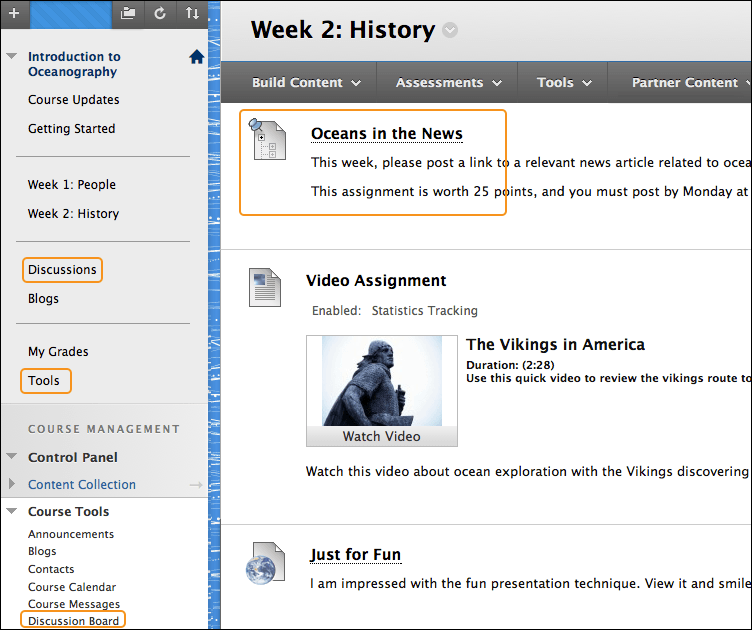
\includegraphics[width=0.7\textwidth]{sections/blackboard/images/discussions_access.png}
	\caption{Accessing Blackboard discussions.}
	\end{figure}
	
You can view the discussion boards using the side \its{Discussions} tab (if it has not been deleted) or using \its{Control Panel} $\to$ \its{Course Tools} $\to$ \its{Discussion Board}. To create a discussion forum:
	
	\begin{enumerate}[1.]
	\item \its{Control Panel} $\to$ \its{Discussions}.
	\item Click \its{Create Forum}. 
	\item Add your content, and choose your options based on the assignment and click \its{Submit}. 
	\end{enumerate} 

Creating discussion sections, forums, and threads is not technically difficult but has lots of possible variation based on the type of assignment and the level of control/interaction the instructor/teaching assistant wants the students to possess. You can find more about all these issues at the following links:
	
	\begin{itemize}
	\item Blackboard Create Discussions: \url{https://help.blackboard.com/Learn/Instructor/Interact/Discussions/Create_Discussions}
	\item Blackboard Create Forums: \url{https://help.blackboard.com/Learn/Instructor/Interact/Discussions/Create_Discussions/Create_Forums}
	\item Blackboard Create Threads: \url{https://help.blackboard.com/Learn/Instructor/Interact/Discussions/Create_Discussions/Create_Threads}
	\item Blackboard Using Discussions in the Original View---YouTube: \url{https://www.youtube.com/watch?v=vNMO-4I7uBI}
	\item Blackboard Create a Discussion---YouTube: \url{https://www.youtube.com/watch?v=q4HDNzZeFqE}
	\end{itemize}



% Copying Your Course
\subsection{Copying Your Course}

You can copy an old course to a new course. This is especially useful when you are teaching the same or a similar course and you will be using much of the same setup or material. To copy a course, do the following:
	
	\begin{enumerate}[1.]
	\item Open the course you wish to copy.
	\item \its{Control Panel} $\to$ \its{Packages and Utilities} $\to$ \its{Course Copy}
	\item Under \its{Select Copy Type}, select ``Copy Course Materials into an Existing Course.''
	\item In the \its{File Attachments} section, select the content you would like to copy.
	\item Click \its{Submit}.
	\end{enumerate}
	
	\begin{figure}[!ht]
	\centering
	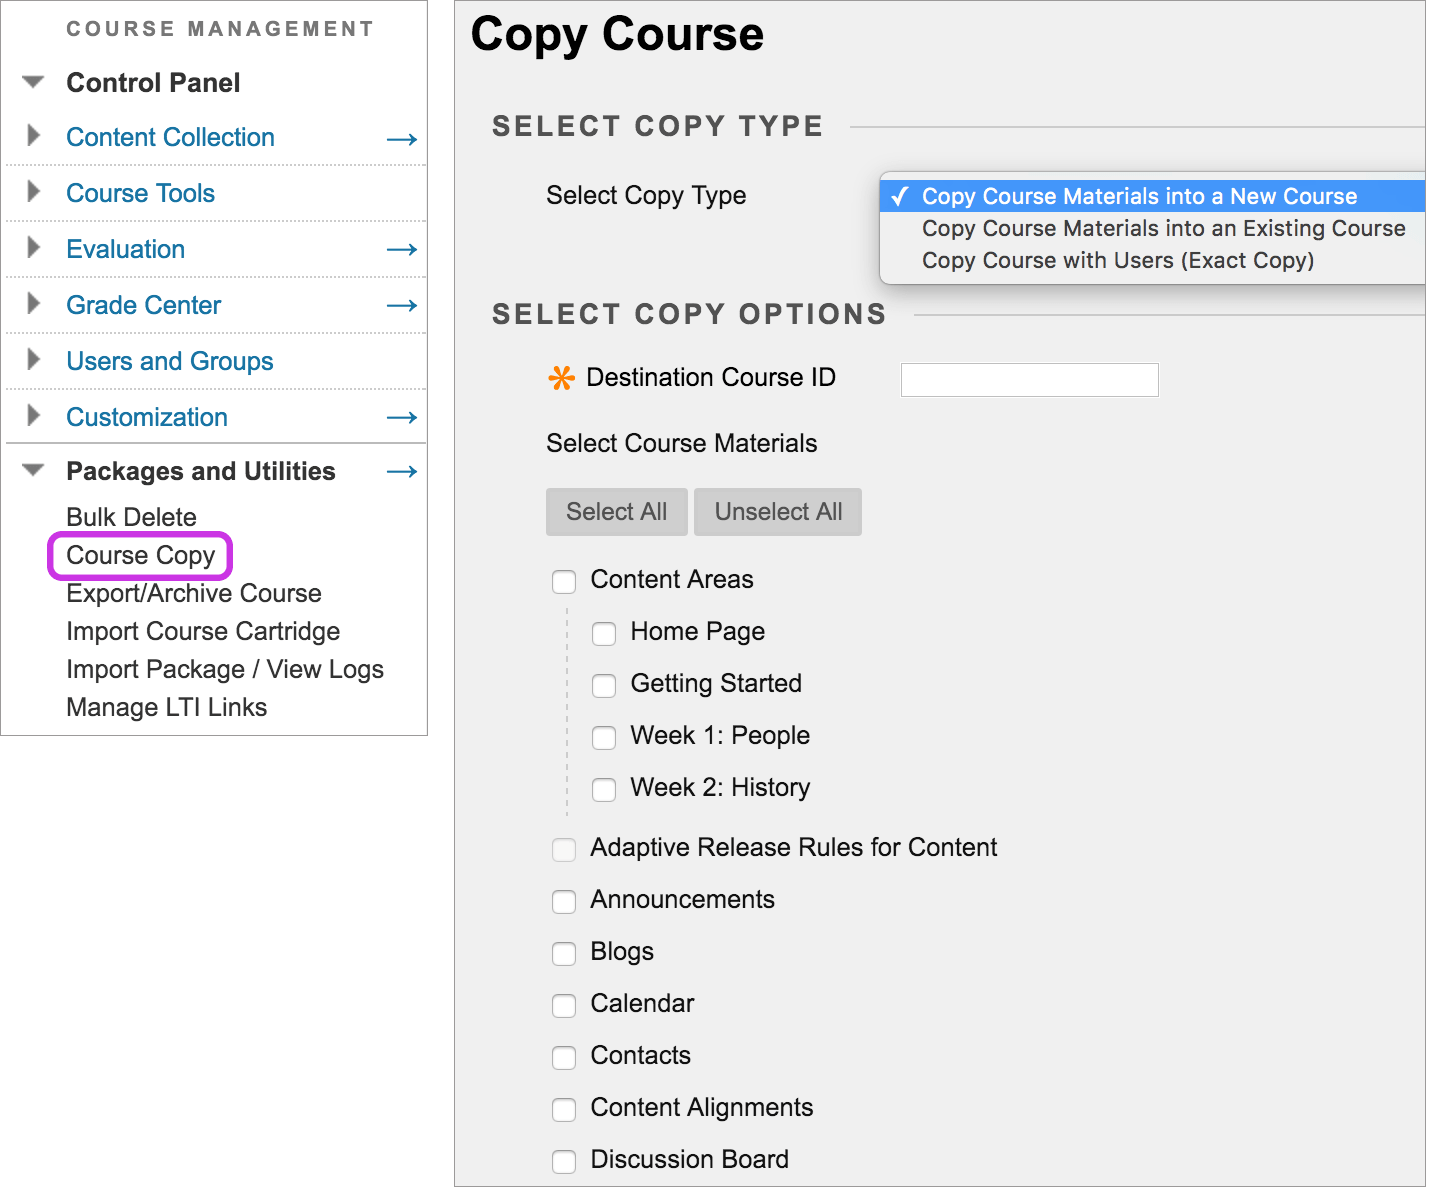
\includegraphics[width=0.7\textwidth]{sections/blackboard/images/original_copy_course.png}
	\caption{Copying course content.}
	\end{figure}

Note that attendance data is not included when you copy a course into a new/existing course. For more information on what is/is not copied along with more information on copying course materials can be found at \url{https://help.blackboard.com/Learn/Instructor/Course_Content/Reuse_Content/Copy_Courses}. 



% Create Content
\subsection{Create Content}

You can add content to your Blackboard course: files, audio, images, video, etc. To add content to your Blackboard course:

	\begin{enumerate}[1.]
	\item \its{Control Panel} $\to$ \its{Content}
	\item Under the \its{Build Content} Tab, select the desired content type.
	\item Provide the necessary entries.
	\item Select \its{Submit}.
	\end{enumerate}

	\begin{figure}[!ht]
	\centering
	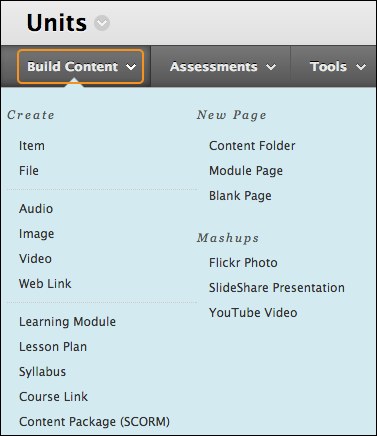
\includegraphics[width=0.5\textwidth]{sections/blackboard/images/build_content_drop_down_list.png}
	\caption{Adding content to Blackboard.}
	\end{figure}

Whenever possible, you should provide accessibility features, such as alternative text, to help students who may require additional accessibility options in order to use the materials. Also consider this when you add items like PDFs, PowerPoints, YouTube videos, etc. You can also add special conditions on when materials become available to students such as required scores on assignments. For more on all these options and abilities, read more below:

	\begin{itemize}
	\item Blackboard Create Content: \url{https://help.blackboard.com/Learn/Instructor/Course_Content/Create_Content}
	\item Setting Release Options: \url{https://help.blackboard.com/Learn/Instructor/Course_Content/Release_Content}
	\end{itemize}



% Creating Assignments
\subsection{Creating Assignments/Surveys}

You can create assignments and surveys in Blackboard. 

	\begin{figure}[!ht]
	\centering
	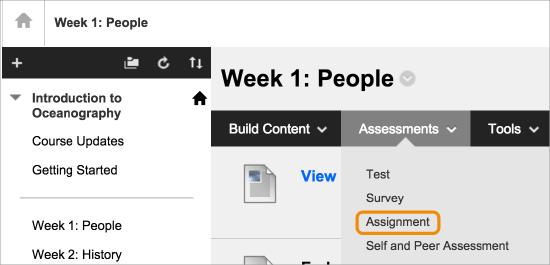
\includegraphics[width=0.8\textwidth]{sections/blackboard/images/assignment_access_original.png}
	\caption{Creating assignments and surveys in Blackboard.}
	\end{figure}

	\begin{enumerate}[1.]
	\item \its{Control Panel} $\to$ \its{Assignments}
	\item Under the \its{Assignments} Tab, select the desired assignment type.
	\item Provide the name, instructions, and any necessary additional files. 
	\item [Optional] Add a due date, any rubrics, and additional options. 
	\item Select \its{Submit}.
	\end{enumerate}

If you assign a due date to an assignment, it automatically shows in the course calendar and in the \its{To Do} module. Assignments submitted after the due date are automatically marked as late, but you may also choose to make the display date the same as the due date so that students cannot submit the assignment late. Assignments also automatically appear in the \its{Gradebook}.

	\begin{figure}[!ht]
	\centering
	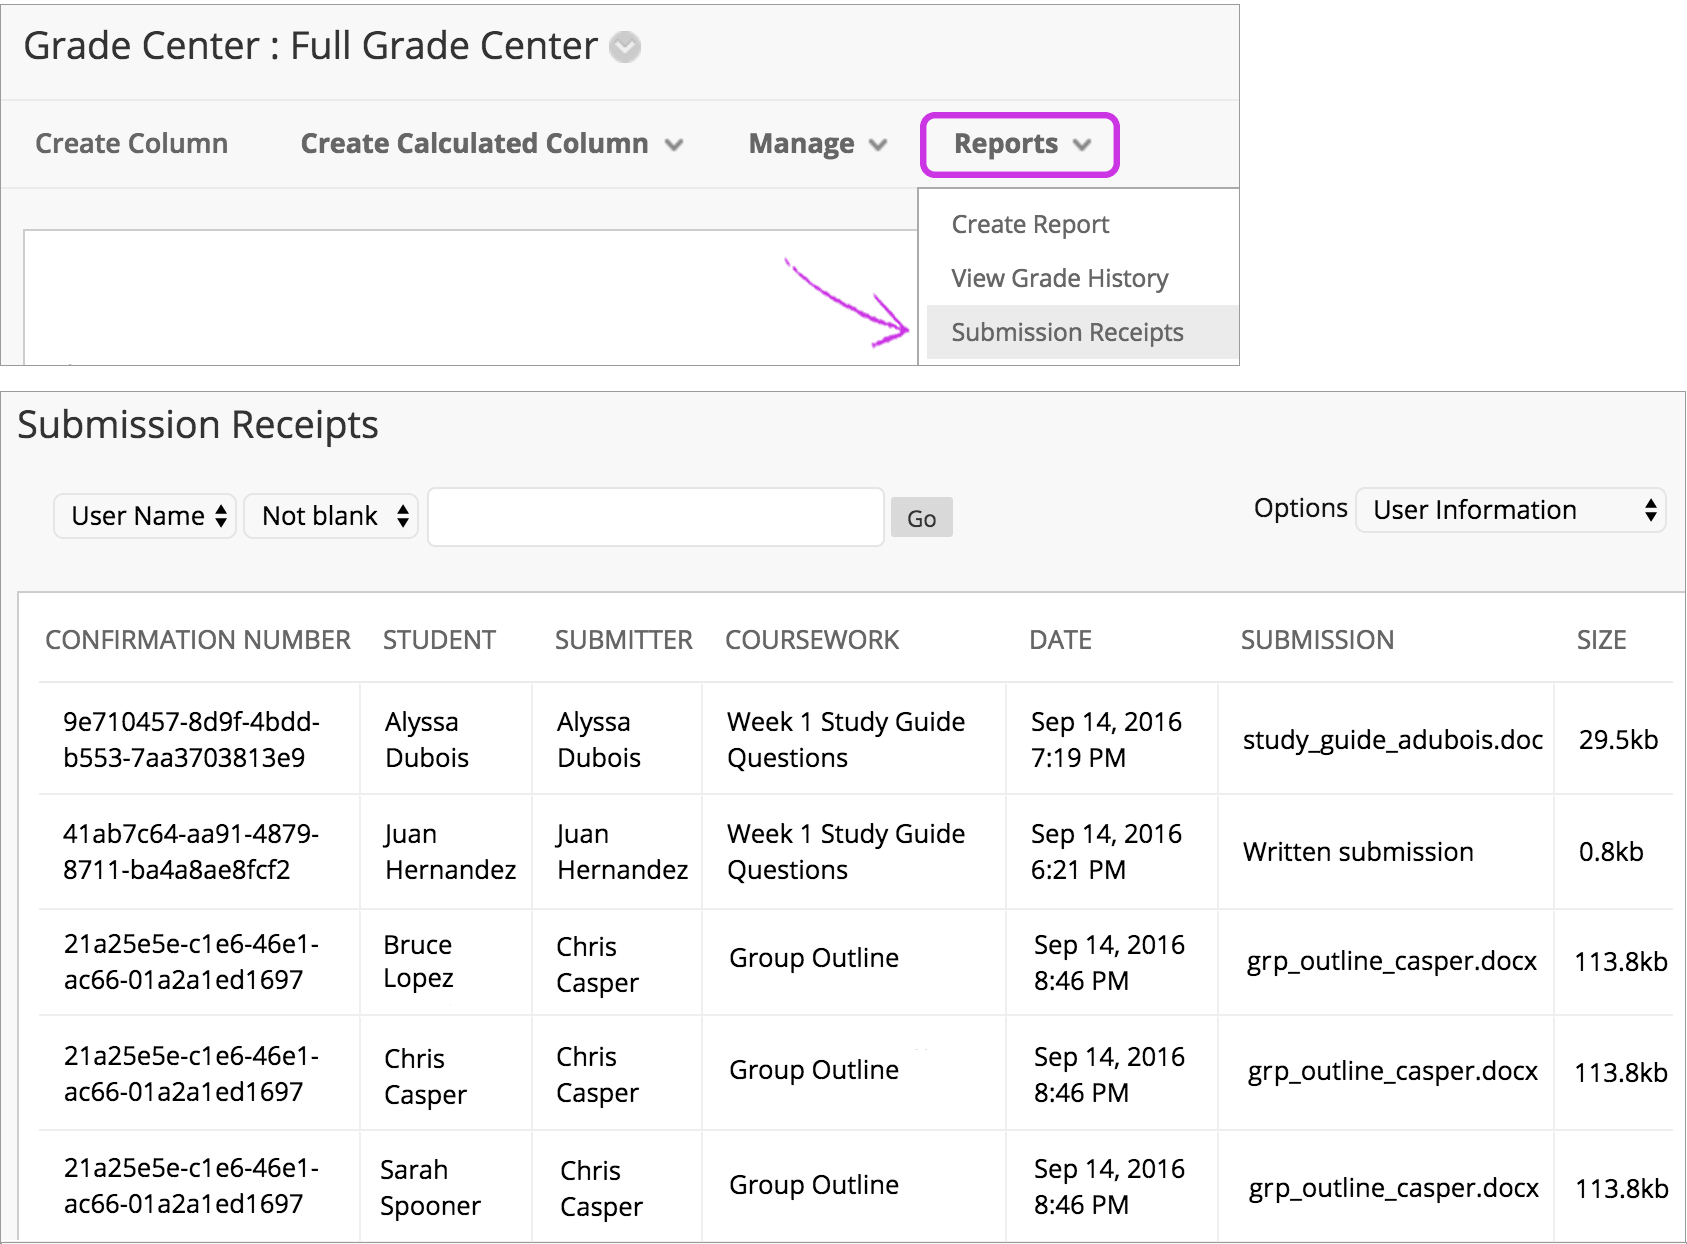
\includegraphics[width=0.9\textwidth]{sections/blackboard/images/original_submission_receipts_grade_center.png}
	\caption{Accessing grade reports.}
	\end{figure}

When students submit an assignment, it also automatically appears in the \its{Needs Grading} section of the \its{Grade Center}. Students can copy and save the confirmation number of their submission as proof of their submission. If multiple submissions are allowed, there is a different confirmation number for each submission. Even if a student deletes a submission, the instructor and administrators always have a retrievable record in the system. You can access all submissions and confirmation numbers from the \its{Reports} tab under \its{Full Grade Center}, which is found under the \its{Grade Center} tab of the \its{Control Panel}.

	\begin{figure}[!ht]
	\centering
	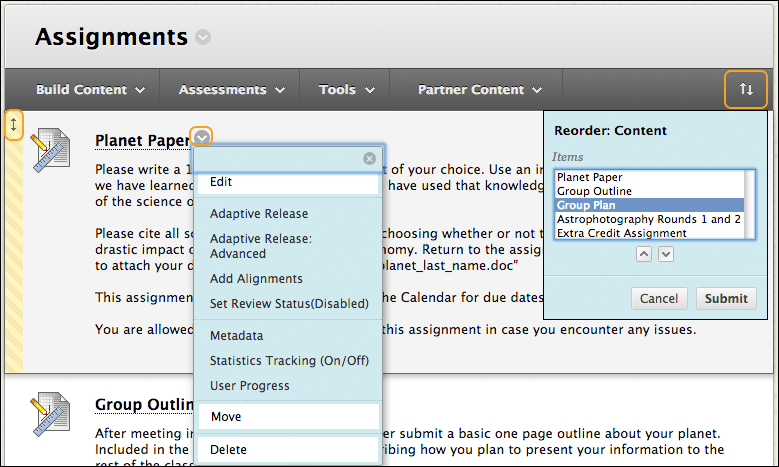
\includegraphics[width=0.9\textwidth]{sections/blackboard/images/edit_assignments_original.png}
	\caption{Reordering assignments.}
	\end{figure}

You have the ability to edit, reorder, and delete any of your assignments. You also can delete assignments. If you delete an assignment for which student submissions already exist, you can either preserve the scores in the \its{Grade Center} while deleting the submissions (you will no longer be able to access them) or delete the assignment, the corresponding \its{Grade Center} column (along with the grades for the submissions), and all the student submissions. These actions are irreversible. Alternatively, you can simply make the item unavailable to students. 

You can find more information along with video on all of the above features below:

	\begin{itemize}
	\item Blackboard Creating Assignments: \url{https://help.blackboard.com/Learn/Instructor/Assignments/Create_and_Edit_Assignments}
	\item Creating Assignments---YouTube: \url{https://www.youtube.com/watch?v=hUXXCp1pnHs}
	\end{itemize}



% Creating Tests
\subsection{Creating Tests}

You can administer tests on Blackboard. Because the topic of creating exams is very specific to the exam you are creating: the number and type of questions, timed or untimed, allowing/disallowing web access, etc., we will not go into the process of creating Blackboard tests but rather provide all the links to the necessary information.

	\begin{itemize}
	\item Blackboard Creating Tests: \url{https://help.blackboard.com/Learn/Instructor/Tests_Pools_Surveys/Create_Tests_and_Surveys}
	\item Creating Tests---YouTube: \url{https://www.youtube.com/watch?v=hms51SQtYzY}
	\item Question Settings: \url{https://help.blackboard.com/Learn/Instructor/Tests_Pools_Surveys/Question_Settings}
	\item Test \& Survey Options: \url{https://help.blackboard.com/Learn/Instructor/Tests_Pools_Surveys/Test_and_Survey_Options}
	\item Deploying Tests: \url{https://help.blackboard.com/Learn/Instructor/Tests_Pools_Surveys/Create_Tests_and_Surveys#deploy}
	\item Test \& Survey Results: \url{https://help.blackboard.com/Learn/Instructor/Tests_Pools_Surveys/Test_and_Survey_Results}
	\end{itemize}





% Gradebook
\subsection{Gradebook}

The \its{Gradebook} allows you to access your students grade and assignment submissions. You access the \its{Gradebook} using the \its{Control Panel}. To view all your students grades and submitted assignments (or those that need grading), select \its{Full Grade Center}.

	\begin{figure}[!ht]
	\centering
	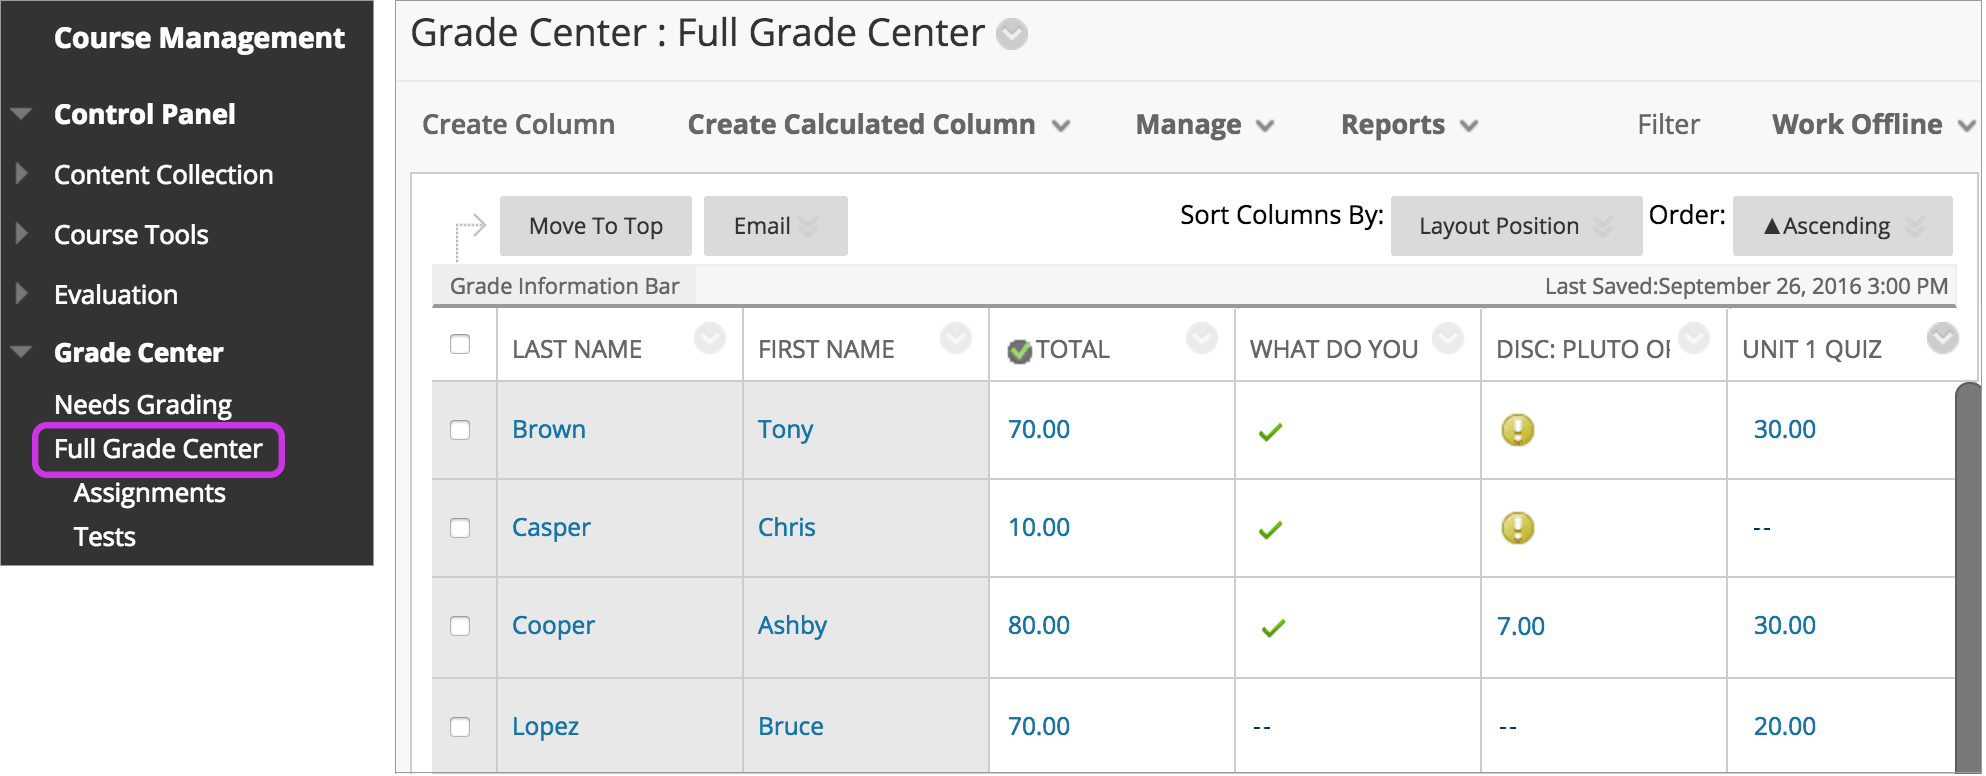
\includegraphics[width=0.9\textwidth]{sections/blackboard/images/original_access_grade_center}
	\caption{Viewing student grades and submissions.}
	\end{figure}

To create a grade column:

	\begin{enumerate}[1.]
	\item Select \its{Create Column}.
	\item Enter a name and description. 
	\item Choose your grading scheme (you can create custom grading schemes).
	\item Enter the points possible. 
	\item Select \its{Submit}.
	\end{enumerate}

Note that when you create a survey, quiz, exam, or other assignment a column is automatically added in the \its{Grade Center}. Assignments which are not yet graded appear in the grade center as a yellow exclamation mark (see the figure above). You can select this cell to grade that students submission. Alternatively, you can view all student submissions which require grading using the \its{Needs Grading} option under the \its{Grade Center} tab in the \its{Control Panel}. You can control also the order of the grade columns for yourself using the \its{Column Organization} option.

You can select whether a grade column is visible to students using the dropdown tab option of the grade column title. From this drop down tab, you can also choose to edit the column after its creation. For instance, you can edit the amount that the assignment is worth. You can download the grade center data. To download grades:

	\begin{enumerate}[1.]
	\item Access the \its{Work Offline} menu and select \its{Download}.
	\item Select the data to download (most likely full grade center).
	\item Select the file type, download location, and whether to download hidden columns.
	\item Select \its{Submit}. 
	\end{enumerate}

You can also use your own gradebook off of Blackboard. You then have two options. First, you could simply create columns such as `Course Average', `Quiz Average', `Participation Grade', etc. and simply update these columns regularly. You can use the rest of the grade center as normal. A second option is to upload your gradebook to Blackboard. However, this requires the gradebook to have specific formatting. We will leave this to the Syracuse University specific link shared below. 

	\begin{itemize}
	\item Blackboard Grading: \url{https://help.blackboard.com/Learn/Instructor/Grade}
	\item Syracuse University---Uploading/Downloading Grades: \url{https://answers.syr.edu/display/blackboard01/Uploading+and+Downloading+Grades}
	\end{itemize}



% Customization
\subsection{Customization}

There are several ways you can customize your Blackboard course page to make it stand out. For instance, you can organize the course menu by renaming, reordering, deleting, hiding, and adding course menu links to fit the course needs. However, deleting a content area link deletes the entire area as well as the items within it, and this action is final. A better option is some cases would be to hide the content area instead. You can read more about the course menu and creating items at this link \url{https://help.blackboard.com/Learn/Instructor/Getting_Started/Navigate_Inside_a_Course}. 


You may also customize the course structure. Most of these course customization options are found under the \its{Control Panel} $\to$ \its{Teaching Style} tab. 

	\begin{figure}[!ht]
	\centering
	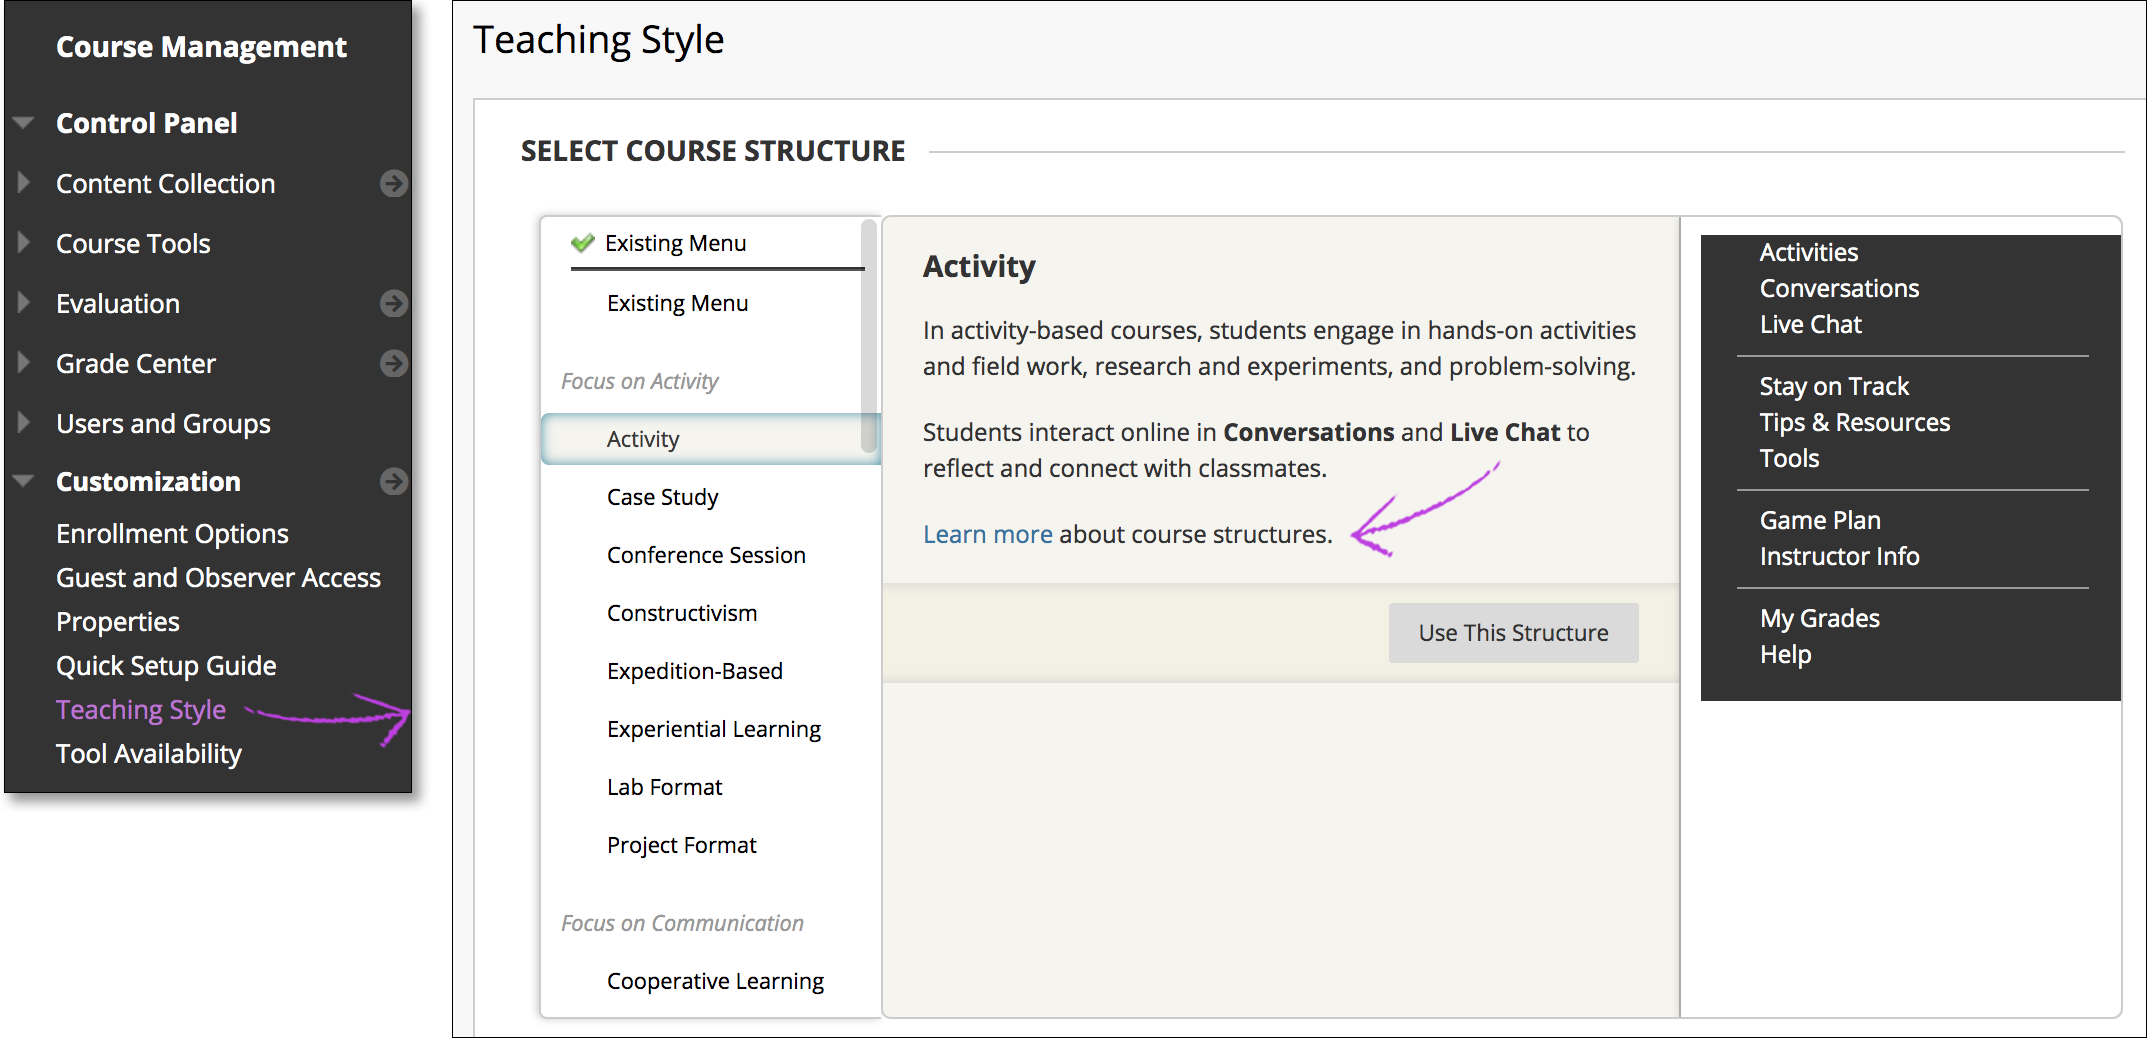
\includegraphics[width=0.9\textwidth]{sections/blackboard/images/orig_instr_course_structure_select_0}
	\caption{Finding the teaching style tab.}
	\end{figure}

For instance, you can choose the first area students will see when they load the course Blackboard page. You may also choose a background image or theme to make your course look more distinctive. This is chosen under the \its{Change Course Theme} option. The menu can also be customized in its color choice, button type, button shape, and button color. This is chosen under the \its{Select Menu Style}. Finally, you can also add banners to your course. You can find out more using the links below:
	
	\begin{itemize}
	\item Blackboard Course Options: \url{https://help.blackboard.com/Learn/Instructor/Courses/Course_Customization/Course_Style_Options}
	\item Blackboard Entry Point---YouTube: \url{https://www.youtube.com/watch?v=RtCKI27Uao4}
	\end{itemize}


You may also choose the Blackboard tools which are available to students. These options are found under the \its{Tool Availability} page. There is also an option for students to have access to Blackboard email features. You may read about these features below:

	\begin{itemize}
	\item Blackboard Tool Availability: \url{https://help.blackboard.com/Learn/Instructor/Courses/Course_Customization/Course_Tool_Availability}
	\item Blackboard Tool Availability---YouTube: \url{https://www.youtube.com/watch?v=665fns0CaMY}
	\end{itemize}

You can also choose a name and description, course classification, course availability, course duration, language pack, etc. For more information on these options, visit \url{https://help.blackboard.com/Learn/Instructor/Courses/Course_Customization/Course_Properties}. You can also read about all of these topics more generally at \url{https://help.blackboard.com/Learn/Instructor/Courses/Course_Customization}. 






% Creating Announncements
\subsection{Creating Emails/Announcements}

You can create announcements or send email some of all of your students in a course via Blackboard. This is done using the \its{Announcements} feature of Blackboard. To send an announcement:

	\begin{enumerate}[1.]
	\item \its{Control Panel} $\to$ \its{Course Tools} $\to$ \its{Announcement}.
	\item Choose \its{Create Announcement}.
	\item Type a subject, which will appear as the subject of the announcement (and email if it is sent). 
	\item Type your message, include any links or images you would like using the tool bar above the message box. 
	\item Choose any date restrictions and whether you want to send an email to all course users or simply post an announcement (the checkbox marked  \its{Send a copy of this announcement immediately.}). 
	\item (Optional) You can use the \its{Course Link} section to link to a course area, tool, or item.
	\item Select Submit.
	\end{enumerate}

If you choose not to send an email to course users, students will still receive a notification on their Blackboard page when they login (assuming they have not turned this feature off). Note that though all the embedded images, videos, links, formatting, attached files, etc. appear as intended when viewing the announcement on the \its{Announcement} page on Blackboard, they may not appear/work as you had intended in the email. 

If there is a mistake in an email or announcement, you may edit the announcement/email or delete it. To edit or delete an announcement, select \its{Edit} or \its{Delete} in its menu. Deleting an announcement is irreversible. If you edit an announcement (whether or not it was originally emailed), you have the option of sending the message via email. In addition, you have the option of 

You also have the ability to send emails from Blackboard to specific users or groups of users. To do this, follow these instructions:

	\begin{enumerate}[1.]
	\item \its{Control Panel} $\to$ \its{Course Tools} $\to$ \its{Send Email}.
	\item Select the desired option, e.g. all users, select groups, select users, etc. 
	\item Send an email starting at step 3 as above. 
	\end{enumerate} 

You can find more resources for sending emails using Blackboard below:

	\begin{itemize}
	\item Blackboard Announcements: \url{https://help.blackboard.com/Learn/Instructor/Interact/Announcements}
	\item Blackboard Email: \url{https://help.blackboard.com/Learn/Instructor/Interact/Email}
	\item Blackboard Creating Announcements---YouTube: \url{https://www.youtube.com/watch?v=UFsPszU0l1k}
	\item Blackboard Sending Email---YouTube: \url{https://www.youtube.com/watch?v=-vdtTB7QC-4}
	\end{itemize}





% Feedback for Students
\subsection{Feedback for Students}

It is possible in Blackboard to record feedback on students submitted work. Feedback can be typed and/or consist of video/audio recordings. When grading an attempt, there will be an arrow to expand the grading screen where you can record written feedback. 

	\begin{figure}[!ht]
	\centering
	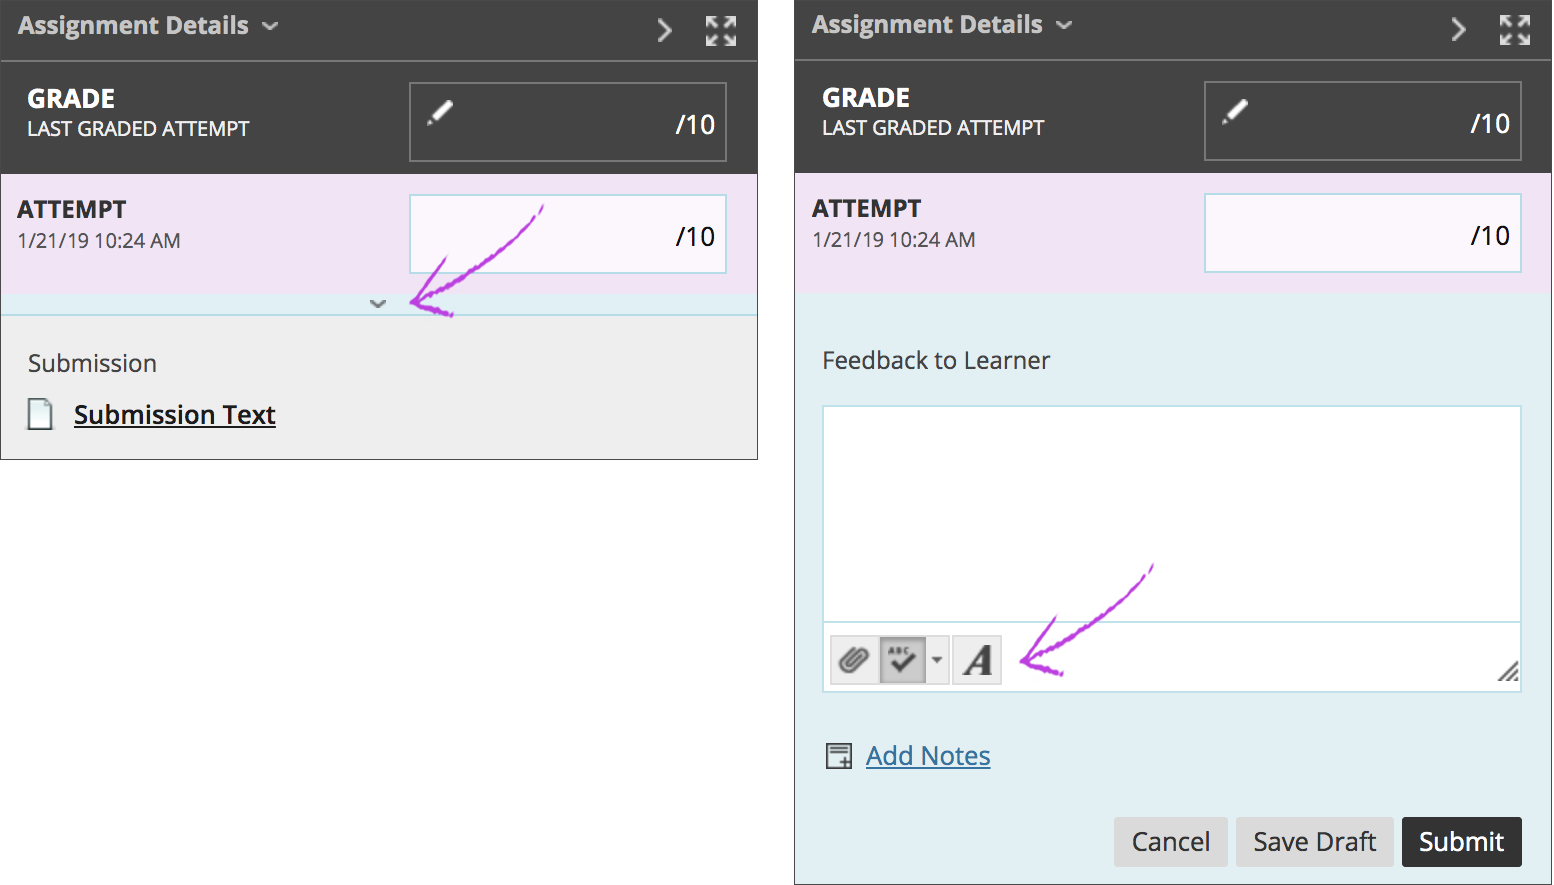
\includegraphics[width=0.9\textwidth]{sections/blackboard/images/orig_instr_open_editor_in_sidebar_0}
	\caption{Feedback on assignment submissions.}
	\end{figure}

In the same window you type your written feedback, you can select the microphone or video recording icon to open a window that allows you to record audio and/or video feedback for your student. You will need to give Blackboard permission to access your computer's microphone and/or camera. Recordings can only be up to five minutes long. Each feedback is unique to the student's submission. You cannot download, share, or reuse feedback recordings. If you want to access feedback you have given a student, you can select the students grade in the \its{Grade Center} and select \its{View Grade Details}. 

	\begin{figure}[!ht]
	\centering
	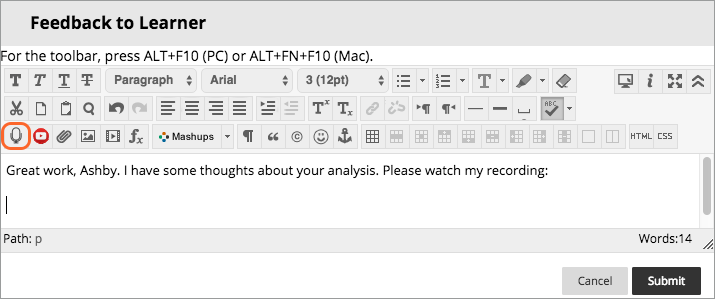
\includegraphics[width=0.9\textwidth]{sections/blackboard/images/original_instructor_feedback_editor}
	\caption{Recording audio/video feedback.}
	\end{figure}
	
Alternatively, one could record video/audio and save it to your computer using the method of your choice and then attach it to the student's grade submission using the option in the window above. This would also be a method to record general feedback for your classes submission. For instance, if many students made a similar mistake, record feedback on the error(s) using a method of your choice, then save the file to your computer. You can then create an announcement (for instance titled `Assignment Name---Feedback') and in announcement attach the audio/video file for students to view. For more information on this topic, see the link below:

	\begin{itemize}
	\item Blackboard Giving Feedback: \url{https://help.blackboard.com/Learn/Instructor/Interact/Audio_Video_Recording}
	\end{itemize}




% Feedback from Students
\subsection{Feedback from Students}

You can also use Blackboard to survey your students for course content/discussions or to receive feedback on an assignment, exam, or general performance. One option is to create a  quiz (worth 0 points if you wish) where you allow students to respond to your survey questions, e.g. extended response or multiple choice based on a Likert scale. This has the advantage of this is being able to assign points for students completing the survey as well as tracking who has/has not completed the survey. 

However more than likely, you will want to make the survey anonymous. Creating anonymous surveys is possible in Blackboard. [If the survey is anonymous, then you will probably want to let the students know, and you may want to consider a test survey and showing the students your view of the results to emphasize the anonymity.] To create a survey:

	\begin{enumerate}[1.]
	\item \its{Control Panel} $\to$ \its{Course Tools} $\to$ \its{Tests, Surveys, and Pools}.
	\item On the survey page, click \its{Build Survey}.
	\item Follow the instructions to create the survey description. Then click \its{Submit}.
	\item Create the survey using \its{Create Question} to enter the questions. 
	\item Click \its{Submit}.
	\end{enumerate}

After creating the survey, you need to deploy the survey. To deploy the survey:

	\begin{enumerate}[1.]
	\item Navigate to the content area where you want the survey to be.
	\item From the \its{Assessments} tab, select \its{Survey}.
	\item On the create survey page, select the survey from the \its{Add Survey} box.
	\item Click \its{Submit}.
	\item Enter the name, description, and options for your survey, including the due date.
	\item Click \its{Submit}.
	\end{enumerate}

For each survey, you can view the aggregate results for each question. To view the results, go to the \its{Grade Center} and click the survey's column action link to access the contextual menu, then select \its{Attempts Statistics}. Surveys in Blackboard are anonymous by default. Alternatively, you can create a survey using Google Forms, Survey Monkey, etc. and link to the survey using a course Announcement. 




% Student Mode
\subsection{Student Preview Mode}

If you are wondering how things look or function from the student end of Blackboard, there is an option for you to view your Blackboard course page as a student. This is called \its{Student Preview Mode}. You access this using an icon in the upper right corner of your Blackboard page. This allows you not only to view the page as a student but interact with the course page as a student. This allows you to perform student activities such as submitting assignments, taking tests, creating blogs/posts, etc. This is different from \its{Edit Mode}, which hides your edit controls and content under certain conditions. The advantage to using \its{Student Preview Mode} is that when exiting the mode, you can save the data from your time in the mode. For example, you can enter student mode, take a quiz, exit student preview mode (saving your data), grade the attempt as the instructor, then re-enter student preview mode to see the grade/grade feedback from the student perspective---among other things. 

	\begin{figure}[!ht]
	\centering
	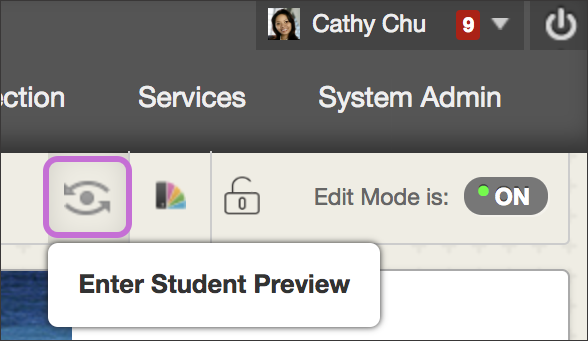
\includegraphics[width=0.45\textwidth]{sections/blackboard/images/orig_instr_student_preview_icon}
	\caption{Entering student preview mode.}
	\end{figure}

You can learn more about this using the links below:

	\begin{itemize}
	\item Blackboard Student Preview Mode: \url{https://help.blackboard.com/Learn/Instructor/Courses/Student_Preview}
	\item Blackboard Student Preview Mode---YouTube: \url{https://www.youtube.com/watch?v=JCrAQewg7Is}
	\end{itemize}



% Collaborate
\subsection{Blackboard Collaborate}

You can use Blackboard to give online lectures, create online person-to-person discussion sessions, etc. This is Blackboard Collaborate. However, there is a session dedicated to using Blackboard Collaborate so we will not go into this in any detail here other than give you a link to read more about Blackboard Collaborate:

	\begin{itemize}
	\item Blackboard Help for Moderators: \url{https://help.blackboard.com/Collaborate/v12/Moderator}
	\end{itemize}






% Track Performance
% https://help.blackboard.com/Learn/Instructor/Performance


% Blogs
% https://help.blackboard.com/Learn/Instructor/Interact/Blogs



% SafeAssign
% Plagarism checks - disclosures
% creating groups https://help.blackboard.com/Learn/Instructor/Interact/Course_Groups/Create_Groups